\definecolor{autodiffSketchForwardFill}{RGB}{255,255,204}
\definecolor{autodiffSketchBackwardFill}{RGB}{161,218,180}

\tikzset{autodiffSketchForward/.style={
    font=\footnotesize,
    fill=autodiffSketchForwardFill,
    thick,
    rounded corners=1ex,
    draw=black,
    minimum width=3.5ex,
    minimum height=3ex,
  }
}

\tikzset{autodiffSketchBackward/.style={
    font=\footnotesize,
    fill=autodiffSketchBackwardFill,
    thick,
    rounded corners=1ex,
    draw=black,
    minimum width=3.5ex,
    minimum height=3ex,
  }
}

\tikzset{autodiffSketchArrow/.style={
    ->,
    >=stealth,
    ultra thick,
    black,
  }
}

\newcommand{\autodiffSketchDrawNodes}{
  \node [anchor = south west, autodiffSketchForward] (z1)
  at (0, 0) {$z^{(1)}$};
  \node [anchor = south east, autodiffSketchForward] (z2)
  at (\figwidth pt, 0) {$z^{(2)}$};
  \node [anchor = center, autodiffSketchForward] (z3)
  at (0.5*\figwidth pt, 0.25*\figheight pt) {$z^{(3)}$};
  \node [anchor = west, autodiffSketchForward] (z4)
  at (0, 0.575*\figheight pt) {$z^{(4)}$};
  \node [anchor = east, autodiffSketchForward] (z5)
  at (\figwidth pt, 0.425*\figheight pt) {$z^{(5)}$};
  \node [anchor = east, autodiffSketchForward] (z6)
  at (\figwidth pt, 0.75*\figheight pt) {$z^{(6)}$};
  \node [anchor = north, autodiffSketchForward] (z7)
  at (0.5*\figwidth pt, \figheight pt) {$z^{(7)}$};
}

\newcommand{\autodiffSketchConnectNodes}{
  \draw[autodiffSketchArrow] (z1.north) to (z4.south);
  \draw[autodiffSketchArrow] (z2.north west) to (z3.south east);
  \draw[autodiffSketchArrow] (z2.north) to (z5.south);
  \draw[autodiffSketchArrow] (z3.north east) to (z5.south west);
  \draw[autodiffSketchArrow] (z4.north) to (z7.south west);
  \draw[autodiffSketchArrow] (z4.north east) to (z6.south west);
  \draw[autodiffSketchArrow] (z5.north) to (z6.south);
  \draw[autodiffSketchArrow] (z6.north west) to (z7.south east);
}

\newcommand{\autodiffSketchDrawBackwardNodes}{
  \draw[autodiffSketchArrow, draw=none] (z1.north) to
  node [midway, autodiffSketchBackward, xshift=2ex] {$\exp(z^{(1)})$}
  (z4.south);
  \draw[autodiffSketchArrow, draw=none] (z2.north west) to
  node [midway, autodiffSketchBackward] {$\cos(z^{(2)})$}
  (z3.south east);
  \draw[autodiffSketchArrow, draw=none] (z2.north) to
  node [midway, autodiffSketchBackward] {$1$}
  (z5.south);
  \draw[autodiffSketchArrow, draw=none] (z3.north east) to
  node [midway, autodiffSketchBackward] {$1$}
  (z5.south west);
  \draw[autodiffSketchArrow, draw=none] (z4.north)
  to
  node [midway, autodiffSketchBackward] {$1$}
  (z7.south west);
  \draw[autodiffSketchArrow, draw=none] (z4.north east) to
  node [midway, autodiffSketchBackward] {$z^{(5)}$}
  (z6.south west);
  \draw[autodiffSketchArrow, draw=none] (z5.north) to
  node [midway, autodiffSketchBackward] {$z^{(4)}$}
  (z6.south);
  \draw[autodiffSketchArrow, draw=none] (z6.north west) to
  node [midway, autodiffSketchBackward] {$1$}
  (z7.south east);
}

\newcommand{\autodiffSketchDefineSizeClip}{
  \pgfmathsetmacro{\figwidth}{0.95\linewidth}
  \pgfmathsetmacro{\figheight}{1.3\linewidth}
  \clip (0,0) rectangle (\figwidth pt, \figheight pt);
}

\begin{figure}
  \centering
  \begin{subfigure}[t]{0.45\linewidth}
    \centering
    \caption{Function as Python program}
    \label{subfig:background::AutodiffSketch1}
\begin{lstlisting}[language=Python]
from math import exp, sin

def z7(z1: float, z2: float):
    """Example function."""

    # intermediate variables
    z3 = sin(z2)
    z5 = z3 + z2
    z4 = exp(z1)
    z6 = z4 * z5

    # output variable
    z7 = z4 + z6

    return z7
\end{lstlisting}
  \end{subfigure}
  \hfill
  \begin{subfigure}[t]{0.45\linewidth}
    \centering
    \caption{Computation graph}
    \label{subfig:background::AutodiffSketch2}
    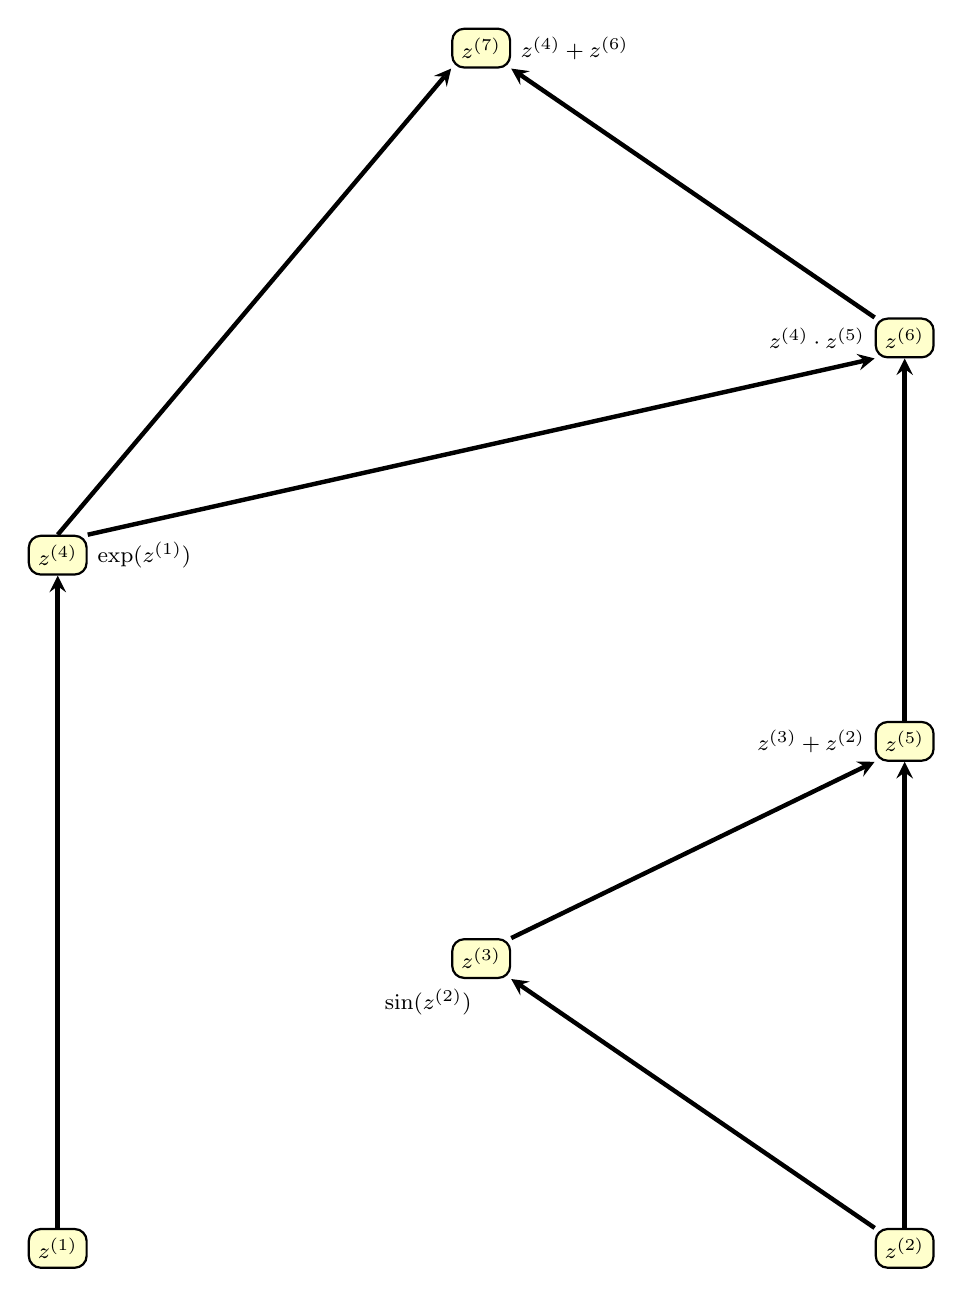
\begin{tikzpicture}
      \autodiffSketchDefineSizeClip
      \autodiffSketchDrawNodes
      \autodiffSketchConnectNodes

      \node [font=\footnotesize, anchor=west] at (z4.east) {$\exp(z^{(1)})$};
      \node [font=\footnotesize, anchor=north east] at (z3.south) {$\sin(z^{(2)})$};
      \node [font=\footnotesize, anchor=east] at (z5.west) {$z^{(3)} + z^{(2)}$};
      \node [font=\footnotesize, anchor=east] at (z6.west) {$z^{(4)} \cdot z^{(5)}$};
      \node [font=\footnotesize, anchor=west] at (z7.east) {$z^{(4)} + z^{(6)}$};
    \end{tikzpicture}
  \end{subfigure}

  \vspace{1ex}

  \begin{subfigure}[t]{0.45\linewidth}
    \centering
    \caption{Local derivatives}
    \label{subfig:background::AutodiffSketch3}
    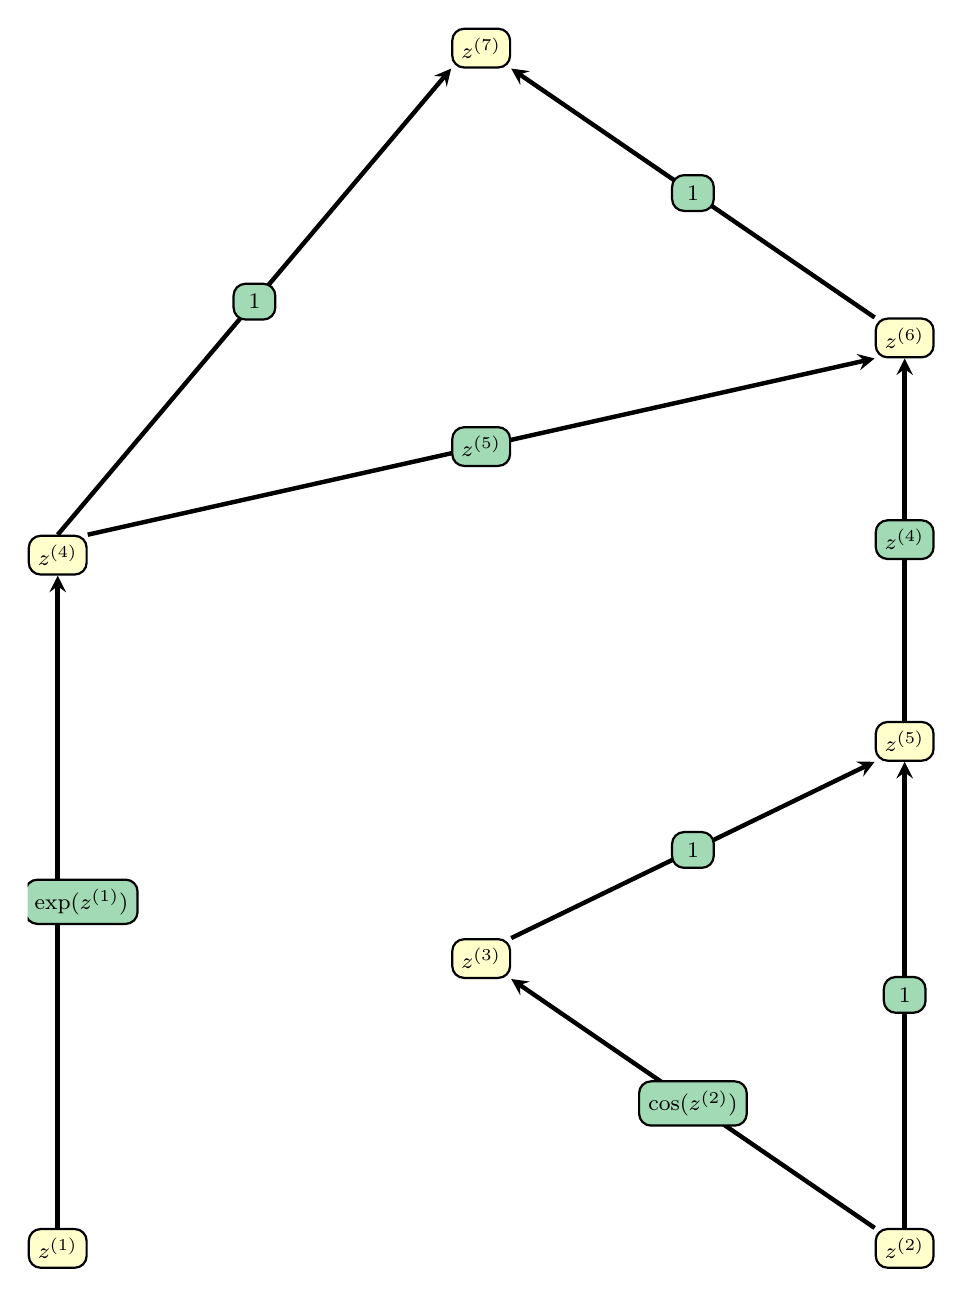
\begin{tikzpicture}
      \autodiffSketchDefineSizeClip
      \autodiffSketchDrawNodes
      \autodiffSketchConnectNodes
      \autodiffSketchDrawBackwardNodes
    \end{tikzpicture}
  \end{subfigure}
  \hfill
  \begin{subfigure}[t]{0.45\linewidth}
    \centering
    \caption{Bauer paths}
    \label{subfig:background::AutodiffSketch4}
    \begin{tikzpicture}
      \autodiffSketchDefineSizeClip

      \begin{scope}[transparency group, opacity=0.2]
        \autodiffSketchDrawNodes
        \autodiffSketchConnectNodes
      \end{scope}
      \begin{scope}[transparency group, opacity=0.66]
        \autodiffSketchDrawBackwardNodes
      \end{scope}

      \begin{pgfonlayer}{background}
        \draw [maincolor, line width = 2.5pt] plot [smooth] coordinates
        {($(z7.east)!0.8!(z7.west)$)
          ($(z4.east)!0.66!(z4.west)$)
          ($(z1.east)!0.66!(z1.west)$)};

        \draw [secondcolor, line width = 2.5pt] plot [smooth] coordinates
        {($(z7.east)!0.6!(z7.west)$)
          ($(z6.east)!0.75!(z6.west)$)
          ($(z4.east)!0.33!(z4.west)$)
          ($(z1.east)!0.33!(z1.west)$)};

        \draw [thirdcolor, line width = 2.5pt] plot [smooth] coordinates
        {($(z7.east)!0.4!(z7.west)$)
          ($(z6.east)!0.5!(z6.west)$)
          ($(z5.east)!0.66!(z5.west)$)
          (z3)
          ($(z2.east)!0.66!(z2.west)$)};

        \draw [darkgraycolor, line width = 2.5pt] plot [smooth] coordinates
        {($(z7.east)!0.2!(z7.west)$)
          ($(z6.east)!0.25!(z6.west)$)
          ($(z5.east)!0.33!(z5.west)$)
          ($(z2.east)!0.33!(z2.west)$)};
      \end{pgfonlayer}
    \end{tikzpicture}
  \end{subfigure}
  \caption{\textbf{Basic AD principles~\cite{oktay2021randomized}.}
    \subfigref{subfig:background::AutodiffSketch1} Example input program
    represented by Python code. The atomic operations combined via
    composition are addition, multiplication, exponential function, and sine.
    The result $z^{(7)}$ is computed from the inputs $z^{(1)}, z^{(2)}$ through
    intermediates $z^{(3)}, z^{(4)}, z^{(5)}, z^{(6)}$,
    \begin{align*}
      z^{(7)}
      &=
        \exp(z^{(1)})
      \\
      &\phantom{=}\,
        + \exp(z^{(1)}) \left( \sin(z^{(2)}) + z^{(2)} \right)\,.
    \end{align*}
    \subfigref{subfig:background::AutodiffSketch2}
    Representation as computation graph to track dependencies between the
    intermediate variables on the level of atomic operations.
    \subfigref{subfig:background::AutodiffSketch3} Computing derivatives relies
    on local derivatives $\nicefrac{\partial z^{(j)}}{\partial z^{(i)}}$ on edges
    $(z^{(i)}, z^{(j)})$, which need to be accumulated according to the chain rule.
    \subfigref{subfig:background::AutodiffSketch4} Interpretation of the chain
    rule as sum over path products. Computing the derivatives of a node \wrt to
    another node in the graph requires summing the path product of local
    derivatives for all paths that connect them. In detail:
    \begin{align*}
      \frac{\partial z^{(7)}}{\partial z^{(1)}}
      &=
        \textcolor{maincolor}{
        \frac{\partial z^{(7)}}{\partial z^{(4)}}
        \frac{\partial z^{(4)}}{\partial z^{(1)}}
        }
        +
        \textcolor{secondcolor}{
        \frac{\partial z^{(7)}}{\partial z^{(6)}}
        \frac{\partial z^{(6)}}{\partial z^{(4)}}
        \frac{\partial z^{(4)}}{\partial z^{(1)}}
        }
      \\
      &=
        \textcolor{maincolor}{
        \exp(z^{(1)})
        }
        +
        \textcolor{secondcolor}{
        z^{(5)}
        \exp(z^{(1)})
        }
      \\
      &=
        \textcolor{maincolor}{
        \exp(z^{(1)})
        }
      \\
      &\phantom{=}\,
        +
        \textcolor{secondcolor}{
        \left( \sin(z^{(2)}) + z^{(2)} \right)
        \exp(z^{(1)})
        }\,,
      \\
      \frac{\partial z^{(7)}}{\partial z^{(2)}}
      &=
        \textcolor{thirdcolor}{
        \frac{\partial z^{(7)}}{\partial z^{(6)}}
        \frac{\partial z^{(6)}}{\partial z^{(5)}}
        \frac{\partial z^{(5)}}{\partial z^{(3)}}
        \frac{\partial z^{(3)}}{\partial z^{(2)}}
        }
      \\
      &\phantom{=}\,
        +
        \textcolor{darkgraycolor}{
        \frac{\partial z^{(7)}}{\partial z^{(6)}}
        \frac{\partial z^{(6)}}{\partial z^{(5)}}
        \frac{\partial z^{(5)}}{\partial z^{(2)}}
        }
      \\
      &=
        \textcolor{thirdcolor}{
        z^{(4)}
        \cos(z^{(2)})
        }
        +
        \textcolor{darkgraycolor}{
        z^{(4)}
        }
      \\
      &=
        \textcolor{thirdcolor}{
        \exp(z^{(1)})
        \cos(z^{(2)})
        }
        +
        \textcolor{darkgraycolor}{
        \exp(z^{(1)})
        }\,.
    \end{align*}}\label{fig:background::AutodiffSketch}
\end{figure}

%%% Local Variables:
%%% mode: latex
%%% TeX-master: "../../thesis"
%%% End:
